\documentclass[oneside, a4paper, 11pt]{memoir}

\usepackage[danish]{babel}        % for Danish metatext
\usepackage{graphicx}             % for figures
\usepackage[chapter]{minted}      % for code highlighting
\usepackage{csquotes}             % for proper quotation marks
\usepackage{caption}              % to better control captions
\usepackage{fontspec}             % for font specification
\usepackage{textcomp}             % for special symbols
\usepackage{fontawesome5}         % for FA icons
\usepackage{relsize}              % for specifying relative font sizes
\usepackage{titlesec}             % to better control section headings
\usepackage{xcolor,pagecolor}     % for coloring links and page backgrounds
\usepackage[hidelinks]{hyperref}  % to make links between sections etc.
\usepackage{enumitem}             % to style lists
\usepackage{pdfpages}             % to include cover page
\usepackage{amsmath}              % for math symbols
\usepackage[
  protrusion=true,
  expansion=true,
  tracking=true
  ]{microtype}                    % to address overflowing margins
\usepackage[
  url=true,
  style=apa
  ]{biblatex}                     % for literature references

\usepackage{etoolbox}
\pretocmd{\section}{\clearpage}{}{}

\addbibresource{../komposition-og-lydproduktion-med-supercollider/bib_assets/klsc.bib}

% Font settings
\setmainfont{Source Sans Pro}
\setmonofont[Contextuals={Alternate}]{Fira Code}

% Page background colors
\definecolor{exercise}{rgb}{0.89, 1, 0.87}
\definecolor{cheatsheet}{rgb}{0.9, 0.9, 1}
\definecolor{normal}{rgb}{1, 1, 1}

% Layout setup
\chapterstyle{veelo}
\hangsecnum
\setsecheadstyle{\Large\bfseries}
\setsubsecheadstyle{\large\bfseries}
\setsubsubsecheadstyle{\normalsize\bfseries}
\setsecnumdepth{subsubsection}

\parindent=0pt
\parskip=1em
\setlength\bibitemsep{\itemsep}

\captionsetup{skip=0.5em, font=footnotesize}

\clubpenalty=10000  % Avoid orphans
\widowpenalty=10000 % Avoid widows
\displaywidowpenalty=10000

\copypagestyle{chapter}{plain}
\makeevenfoot{ruled}{}{\footnotesize\thepage}{}
\makeoddfoot{ruled}{}{\footnotesize\thepage}{}
\makeevenfoot{chapter}{}{\footnotesize\thepage}{}
\makeoddfoot{chapter}{}{\footnotesize\thepage}{}

% For most of the frontmatter
\copypagestyle{ruled_no_footer}{ruled}
\makeevenfoot{ruled_no_footer}{}{}{}
\makeoddfoot{ruled_no_footer}{}{}{}


% Settings for code listings
\definecolor{code_bg}{rgb}{0.95, 0.955, 0.945} % code block background color
\definecolor{code_hl}{rgb}{0.85, 0.92, 0.85} % code block highlight color
\setminted{
  style=friendly,
  frame=single,
  framesep=1mm,
  framerule=1pt,
  xleftmargin=0em,
  xrightmargin=0em,
  numbersep=0.6em,
  linenos=true,
  bgcolor=code_bg,
  bgcolorpadding=0.5em,
  breaklines=true,
  highlightcolor=code_hl,
  ignorelexererrors=true,
  fontsize=\footnotesize,
}
\setmintedinline{
  bgcolor=none,
  style=friendly,
  breaklines=true,
  breakanywhere=true,
  breakautoindent=true,
  fontsize=\relsize{-1}
}
\AtBeginEnvironment{minted}{\setlength{\parskip}{0pt}}

\renewcommand{\listingscaption}{Kodeboks}
\renewcommand{\listoflistingscaption}{Kodebokse}
\renewcommand{\listoflistings}{
  \clearpage
  \phantomsection
  \addcontentsline{toc}{chapter}{\listoflistingscaption}
  \listof{listing}{\listoflistingscaption}
}

\DeclareRobustCommand{\sbseries}{\fontseries{sb}\selectfont}
\DeclareTextFontCommand{\textsb}{\sbseries}


% List settings
\setlist{noitemsep}
\setlist[description]{style=nextline}
\renewcommand{\descriptionlabel}[1]{\textsc{#1}}

\setlist[itemize]{leftmargin=1.7em, labelindent=0pt, label=\faAngleRight}
\setlist[enumerate]{leftmargin=1.7em, labelindent=0pt}
\AtBeginEnvironment{itemize}{\setlength{\parskip}{0.1em}}
\AtBeginEnvironment{enumerate}{\setlength{\parskip}{0.1em}}

% Metadata
\title{Komposition og lydproduktion med SuperCollider}
\author{Anders Eskildsen}

% Misc
\hfuzz=2pt
\vfuzz=2pt

\hypersetup{
  bookmarksnumbered,
  % Black links for TOC
  colorlinks,
  linkcolor={black},
  citecolor={black},
  urlcolor={black}
}

\setcounter{tocdepth}{2}

\makeatletter
\renewcommand{\cleartooddpage}{
  \clearpage
  \ifodd\c@page
      % Already on odd page, do nothing
  \else
    \pagecolor{normal}
    \thispagestyle{empty}
    \hbox{}
    \newpage
  \fi
}
\makeatother

\newcommand{\insertblankpage}{
\newpage
\thispagestyle{empty}
~
\newpage
}

\AtBeginDocument{\addtocontents{toc}{\protect\thispagestyle{empty}}} 

\begin{document}


\includepdf{book_media/coverpage.pdf}

\insertblankpage

% Title page
\thispagestyle{empty}

\begin{center}
  \vspace*{1.5cm}
  {\bfseries
  {\Large \theauthor}
  \vfill
  {\huge \thetitle}
  }
  \vfill
  
\includegraphics[width=0.35\textwidth]{book_media/OPEN_CENTER_BLACK.eps}
\end{center}

% Kolofon
\thispagestyle{empty}

\vspace{4em}
\emph{Komposition og lydproduktion med SuperCollider} \\
Af Anders Eskildsen

1. udgave, 2025 \\
\copyright{} Forfatteren, 2025

Omslag og grafisk layout: Anders Eskildsen

ISBN: 97887-7642-045-1 \\
DOI: 10.54337/aau.kolms2025

Udgivet af: \\
Aalborg University Open Publishing | \href{https://www.open.aau.dk}{www.open.aau.dk}

\vspace{1em}
\href{https://creativecommons.org/licenses/by-sa/4.0/}{\includegraphics[width=0.25\textwidth]{book_media/cc-by-sa.eps}} \\
Dette værk er udgivet under Creative Commons Open Access-licensen \href{https://creativecommons.org/licenses/by-sa/4.0/}{CC BY-SA 4.0}, som tillader andre at distribuere, tilpasse og bygge videre på materialet i ethvert medie eller format, så længe forfatterne krediteres og afledte materialer udgives under samme licens. CC BY-SA 4.0 gælder for værkets indhold, medmindre andet er angivet.


\pagestyle{ruled_no_footer}
\pdfbookmark[1]{Indhold}{toc}
\tableofcontents*
\clearpage
\thispagestyle{empty}

\hypersetup{
  % Use colored links in the main body of the book
  linkcolor={green!40!black},
  citecolor={green!25!black},
  urlcolor={blue!35!black}
}

\frontmatter
\pagestyle{ruled}

\include{chapters/chap99.tex} % preface

\mainmatter

\setcounter{chapter}{-1}

\cleartooddpage
\include{chapters/chap00.tex}
\cleartooddpage
\include{chapters/chap01.tex}
\cleartooddpage
\include{chapters/chap02.tex}
\cleartooddpage
\include{chapters/chap03.tex}
\cleartooddpage
\include{chapters/chap04.tex}
\cleartooddpage
\include{chapters/chap05.tex}
\cleartooddpage
\include{chapters/chap06.tex}
\cleartooddpage
\include{chapters/chap07.tex}
\cleartooddpage
\include{chapters/chap08.tex}
\cleartooddpage
\include{chapters/chap09.tex}
\cleartooddpage
\include{chapters/chap10.tex}

\backmatter

\pagecolor{normal}
\hypersetup{
  % Black links for back matter
  linkcolor={black},
  citecolor={black},
  urlcolor={black}
}

\listoffigures
\listoflistings
\printbibliography[title={Referencer}]


\includepdf{book_media/coverpage-back.pdf}

\end{document}